\documentclass[tcc,capa]{texufpel}

\usepackage[utf8]{inputenc} % acentuacao
\usepackage{graphicx} % para inserir figuras
\usepackage[T1]{fontenc}

\hypersetup{
    hidelinks, % Remove coloração e caixas
    unicode=true,   %Permite acentuação no bookmark
    linktoc=all %Habilita link no nome e página do sumário
}

\unidade{Centro de Desenvolvimento Tecnológico}
\curso{Ciência da Computação}
\nomecurso{Bacharelado em Ciência da Computação}
\titulocurso{Bacharel em Ciência da Computação}

\unidadeeng{Technology Development Center}
\cursoeng{Computer Science}


\title{Visual Sims: uma ferramenta que utiliza Computação Gráfica para auxiliar a aprendizagem}

\author{Sampaio}{Letícia}
\advisor[Prof.~Dr.]{Torchelsen}{Rafael Piccin}
% \coadvisor[Prof.~Dr.]{Aguiar}{Marilton Sanchotene de}
% \collaborator[Prof.~Dr.]{Aguiar}{Marilton Sanchotene de}

%Palavras-chave em PT_BR
\keyword{Computação Gráfica}
\keyword{WebGL}
\keyword{Simulação}
\keyword{Interatividade}

%Palavras-chave em EN_US
\keywordeng{Graphyc Computing}
\keywordeng{WebGL}
\keywordeng{Simulation}
\keywordeng{Interactivity}

\begin{document}

% \renewcommand{\advisorname}{Orientadora}           %descomente caso tenhas orientadora
%\renewcommand{\coadvisorname}{Coorientadora}      %descomente caso tenhas coorientadora

\maketitle 

\sloppy

\fichacatalografica

%\folhadeaprovacao

%Composição da Banca Examinadora
\begin{aprovacao}{18 de junho de 2021} %data da banca por extenso
\noindent Prof. Dr. Rafael Piccin Torchelsen (orientador)\\
Doutor em Ciência da Computação pela Universidade Federal do Rio Grande do Sul.\\[1cm]

\noindent Prof. Dr. Marilton Sanchotene de Aguiar\\
Doutor em Ciência da Computação pela Universidade Federal do Rio Grande do Sul.\\[1cm]

\noindent Profa. Dra. Tatiana Aires Tavares\\
Doutora em Engenharia Elétrica pela Universidade Federal do Rio Grande do Norte.\\[1cm]

\end{aprovacao}

%Opcional
\begin{dedicatoria}
  Gostaria de dedicar este trabalho à comunidade discente dos cursos de Ciência e Engenharia da Computação. Este trabalho é acima de tudo, para a comunidade.
\end{dedicatoria}

%Opcional
\begin{agradecimentos}
  Agradeço primeiramente a minha família, por ter me incentivado a procurar um curso superior e me proporcionar esta experiência. 
  À minha namorada, que me mostrou a importância de se dedicar a tudo que fazemos, sempre dando o nosso melhor.
  Por fim, agradeço ao meu orientador, que continuou trabalhando comigo apesar dos prazos que impus a ele.
\end{agradecimentos}

%Opcional
\begin{epigrafe}
  It's not stupid if it works.\\
  {\sc --- Alunos de computação}
\end{epigrafe}

%Resumo em Portugues (no maximo 500 palavras)
\begin{abstract}
Para alunos dos cursos de Ciência e Engenharia de Computação encontrar conteúdo para estudar é uma tarefa fácil, entretanto existem poucas fontes de pesquisa que disponibilizam um conteúdo interativo. Conceitos ensinados de forma apenas teórica podem surgir como barreira para uma parcela desses alunos, por isso transformar um conteúdo teórico em prático e tornar esse conteúdo acessível é o objetivo deste trabalho. Com isso, proponho um site com exemplos visuais e interativos de conteúdos abordados nas cadeiras de graduação dos cursos de Ciência e Engenharia de Computação. Utilizando conceitos de computação gráfica o aluno poderá visualizar exemplos e aprender de forma mais fácil o conteúdo abordado. Além da versão visual também será disponibilizado uma explicação textual do conteúdo. O site poderá dessa forma ser utilizado como ferramenta para estudo extra classe ou até como uma ferramenta para auxiliar o professor no ensino a distância.
\end{abstract}

%Resumo em Inglês (no maximo 500 palavras)
\begin{englishabstract}{Titulo do Trabalho em Ingles}
Bla blabla blablabla bla.  Bla blabla blablabla bla.  Bla blabla
blablabla bla.  Bla blabla blablabla bla.  Bla blabla blablabla bla.
Bla blabla blablabla bla.  Bla blabla blablabla bla.  Bla blabla
blablabla bla.  Bla blabla blablabla bla.  Bla blabla blablabla bla.
Bla blabla blablabla bla.  Bla blabla blablabla bla.  Bla blabla
blablabla bla.  Bla blabla blablabla bla.  Bla blabla blablabla bla.
Bla blabla blablabla bla.  Bla blabla blablabla bla.  Bla blabla
blablabla bla.  Bla blabla blablabla bla.  Bla blabla blablabla bla.
Bla blabla blablabla bla.
\end{englishabstract}

%Lista de Figuras
\listoffigures

%Lista de Tabelas
\listoftables

%lista de abreviaturas e siglas
\begin{listofabbrv}{ABNT}%coloque aqui a maior sigla para ajustar a distância
        \item[ABNT] Associação Brasileira de Normas Técnicas
        \item[V-Sync] Vertical Synchronization
        \item[WebGL] Web Graphics Library
        \item[OpenGL] Open Graphics Library
        \item[API] Application Programming Interface
        \item[HTML] HyperText Markup Language
        \item[CSS] Cascading Style Sheets
\end{listofabbrv}

%Sumario
\tableofcontents

\chapter{Introdução}
\label{cap: introducao}

Trabalhar com ensino é uma além de passar o conhecimento aos alunos, estar sempre se desafiando e procurando novas formas de ensinar. Assim como a Computação é uma área em constante evolução, novas tecnologias são criadas e devemos nos manter atualizados no que pode nos ajudar e melhorar ainda mais nosso desempenho como profissionais. 

Cada vez mais o mundo virtual invade nossas vidas, já é esperado de nós que o tempo online seja maior que o offline. Além de ser uma grande ferramenta para o ensino, usar a tecnologia para é cada vez mais importante para manter o interesse dos alunos. 

Na área da Computação, a falta de interesse dos alunos por aprender um conteúdo mais difícil é notório e cabe aos professores procurar uma forma de atrair a atenção dos alunos. Ainda na mesma área é comum o interesse por realidades virtuais 

Outro desafio no aprendizado em Computação é a falta de uma infraestrutura que possibilite o aprendizado. Como apontado por~\cite{rauen2003abordagem} em sua pesquisa sobre o ensino de Redes de Computadores, a falta de laboratórios é um dos maiores agravantes para o aprendizado do conteúdo. Entretanto esse cenário não é comum somente ao ensino de Redes, para ensinar  Computação um laboratório bem equipado faz o nível de aprendizado dos alunos crescer.

Como contra proposta aos problemas de infraestrutura temos o uso de simulações voltadas ao ensino. Com elas é possível criar qualquer tipo de situação que facilite a exemplificação de um conceito, sem limitação de espaço ou casualidade de um evento acontecer. 

\section{Objetivos}

O presente trabalho tem como objetivo construir uma plataforma que funciona como galeria para simulações que auxiliem o ensino de conteúdos ligados a Computação. Como parte do objetivo, as simulações devem utilizar elementos gráficos e interativos para ajudar na compreensão, além de ser disponibilizado de forma gratuita e de fácil acesso aos alunos de Ciência e Engenharia de Computação.

\section{Organização do trabalho}

Este trabalho apresenta, no capítulo~\ref{cap: fundamentacao_teorica}, uma breve análise sobre as dificuldades encontradas no ensino, com foco no ensino de Computação, e métodos que outros autores encontraram para resolver este problema. O capítulo~\ref{cap: trabalhos_relacionados} é dedicado aos trabalhos relacionados ao objetivo proposto. Uma breve navegação pelo site desenvolvido está disponível no capítulo~\ref{cap: navegacao}. No capítulo~\ref{cap: desenvolvimento} é apresentado os passos necessários para o resultado final do site proposto. No capítulo~\ref{cap: resultados_e_discussoes} é discutido os resultados do trabalho desenvolvido e o capítulo~\ref{cap: conclusao} encerra este trabalho apresentando a conclusão e uma visão para o que pode ser o futuro deste trabalho.

\chapter{Fundamentação teórica}
\label{cap: fundamentacao_teorica}

Cada individuo tem a sua forma de aprender, bem como cada professor tem a sua forma de ensinar. Por este motivo é essencial que o estudante se prepare previamente e saiba a melhor forma de aprender um novo conhecimento e que o professor esteja aberto aos diferentes tipos de alunos que vai encontrar. Entretanto, os estilos de ensino e aprendizado geralmente não são compatíveis~\cite{felder1988learning}.

Estas duas realidades têm o mesmo objetivo, solidificar o conhecimento do aluno para o desenvolvimento de um bom profissional. Então a busca por métodos inovativos de aprendizado é um tópico recorrente em diversas áreas que envolvem Computação, sempre com o intuito de tornar o conhecimento mais adaptável a realidade do estudante e ajudar o professor a atingir o seu objetivo. Pesquisas  ~\cite{drachsler2015panorama} ~\cite{aguiar2018recomendaccao}

\section{Formas de ensino}

Existem duas grande vertentes do ensino, o Ensino Presencial e o Ensino à Distância. Essas duas formas de passar o conhecimento possuem grandes diferenças e os seus desafios. 

Enquanto o Ensino Presencial, geralmente, se baseia em aulas majoritariamente em formato de palestras, explicações verbais e citações de exemplos, no Ensino Remoto é mais comum os professores basearem o conteúdo em textos e exercícios.

\subsection{Ensino Presencial}

O Ensino Presencial consiste em aulas onde os professores passam o conteúdo aos alunos de forma verbal, em forma de palestra ou debate. Também é comum a apresentação de exemplos de aplicação da matéria proposta. Neste formato não é usual a apresentação de mídias em aula, este padrão é seguido por se acreditar que mídias possam fazer os alunos dispersarem e não passar o conteúdo da forma correta. Entretanto a boa utilização de exemplos visuais têm se mostrado mais apelativo aos olhos dos estudantes.

\subsection{Ensino Remoto}

No Ensino Remoto é comum a utilização de mídias para auxiliar no aprendizado, as próprias aulas são ministradas em ambientes virtuais. Portanto o uso de outras formas de apresentar o conteúdo já está intrínseco no formato remoto. A fixação do conteúdo geralmente se dá por meio de atividades e trabalhos e o aluno está mais inserido ao uso de tecnologias para resolver suas atividades.

Em ambos os âmbitos do ensino, exemplos do conteúdo que o aluno pode interagir e estimula a sua curiosidade têm demonstrado resultados melhores do que apenas ler um livro sobre o assunto.

\section{Simulações no ensino}%não gostei do nome mas por enquanto fica

Utilizar jogos ou simulações como ferramenta de aprendizado é uma tática que se aplica em diversas áreas do aprendizado. 

O uso de simulações para auxiliar o ensino é um tópico que pode ser aplicado em diversas áreas do aprendizado. 

\section{Computação no Ensino}

Guiados por professores, os alunos de Ciência e Engenharia da Computação, têm o objetivo de aprender o conteúdo definido no programa da graduação, já a forma que o conhecimento é passado ao aluno fica por responsabilidade do professor. Para algumas cadeiras é muito difícil explicar a aplicação do conceito sendo passado, por ser um conceito abstrato ou por falta de recursos visuais. Nesses casos os professores podem recorrer a técnicas ou ferramentas que auxiliem os alunos a aprender de forma mais dinâmica o conteúdo.

Uma ferramenta que está muito presente no ensino extra classe é o Ambiente Virtual de Aprendizagem (AVA) que conforme Voss~\cite{Voss_Nunes_Herpich_Medina_2015} é um ambiente que aperfeiçoa a qualidade do ensino dos alunos, por meio de atividades além da sala de aula. Levando em consideração o contexto de ensino a distância, essas ferramentas se tornam essenciais para o desenvolvimento de um ensino de qualidade. 

No contexto computacional é comum aos professores buscarem formas de atrair a atenção dos alunos por meio de exemplos e atividades práticas que sejam interessantes para eles, como jogos e a robótica. Neste contexto simulações podem se tornar outro modo de cativar o interesse dos alunos, por serem aplicáveis para alunos de qualquer nível ou idade, além de retirar a dependência de um ambiente físico para exemplificação de um conteúdo~\cite{kincaid2003simulation}.

O conhecimento é fixado de forma diferente para cada pessoa, porém estímulos visuais se mostram mais eficientes no aprendizado, pois podem explorar de forma lúdica conceitos mais complexos~\cite{klawe1999computer}. Por este motivo o propósito do projeto proposto é fazer com que até as cadeiras que não possuem uma vertente prática possam utilizar de uma ferramenta dinâmica como auxiliar.

\chapter{Trabalhos Relacionados}
\label{cap: trabalhos_relacionados}

Com base em simulações visuais e interativas os alunos podem explorar o que os conteúdos teóricos podem representar. Alguns trabalhos semelhantes já foram desenvolvidos e apresentaram resultado positivo em outros públicos alvo. Um trabalho similar, mas voltado aos alunos de ensino médio, é o site PHET~\cite{phet_2002}. Ele conta com diversas simulações que envolvem física, matemática e química. No site é possível acessar a biblioteca de simulações e interagir com variáveis e ver uma animação representando a mudança que essas variáveis trazem. 

Também temos o livro Immersive Linear Algebra~\cite{strom2017immersive} que conta com modelos em 3D e iterativos que ajudam na fixação e compreensão do conteúdo explicado. Com os modelos disponíveis no livro é possível ver as alterações que as fórmulas implicam nos gráficos e assim entender de forma gradual sua função.

Podemos utilizar o site WebGL Fundamentals~\cite{webgl_2017} também como referência de que contando com exemplos visuais o conteúdo sendo explicado se fixa melhor. No site aprendemos como utilizar a ferramenta WebGL, com exemplos iterativos junto à explicação.

\chapter{Navegação}
\label{cap: navegacao}

Antes de tratar sobre as tecnologias utilizadas é importante termos uma visão do que estamos falando, por isso a seguir serão apresentadas as telas e navegação da plataforma.

Ao abrir a plataforma o usuário já entra em contato com a proposta do site e elementos em 3D, visto na figura~\ref{home}. 

\begin{figure}[htbp]
  \centering 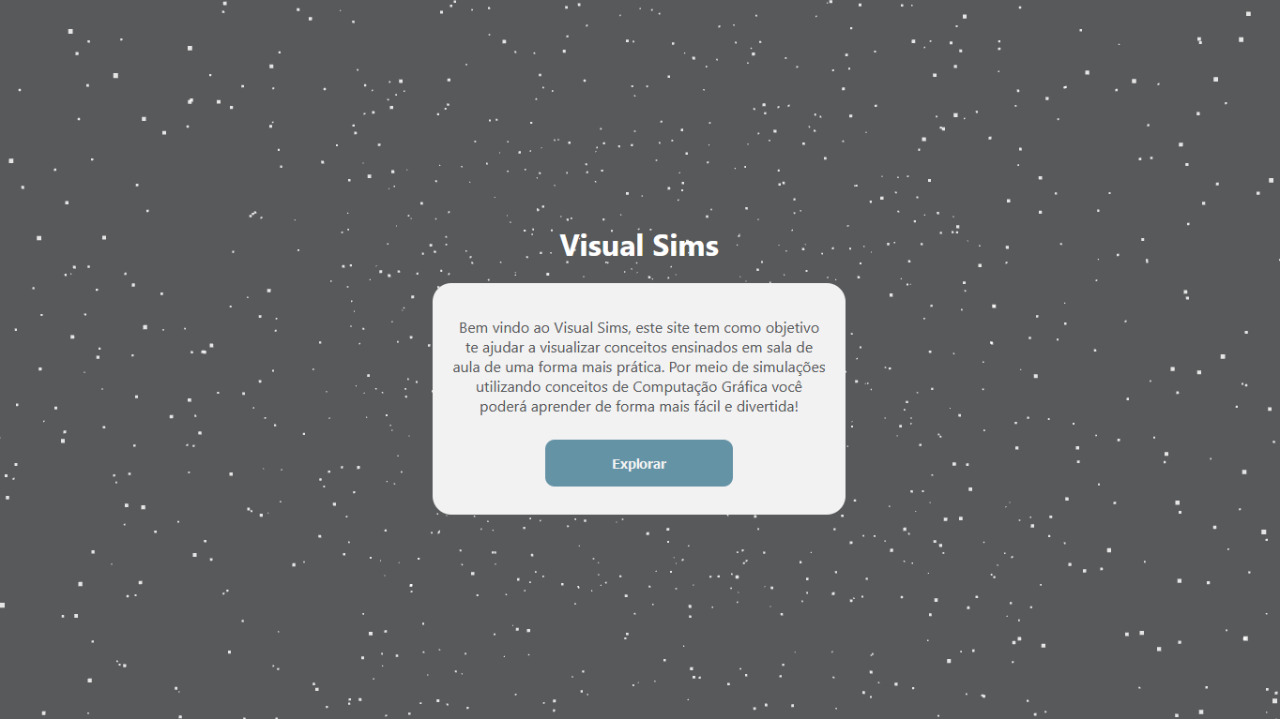
\includegraphics[scale=.2]{Navegacao/pagina_home.jpeg}
  \caption{Página principal}
  \label{home}
\end{figure}

Seguindo o fluxo o usuário entrará na galeria de simulações, figura~\ref{galeria}, onde poderá visualizar mais informações sobre a simulação clicando nela, figura~\ref{card_galeria}.

\begin{figure}[htbp]
  \centering 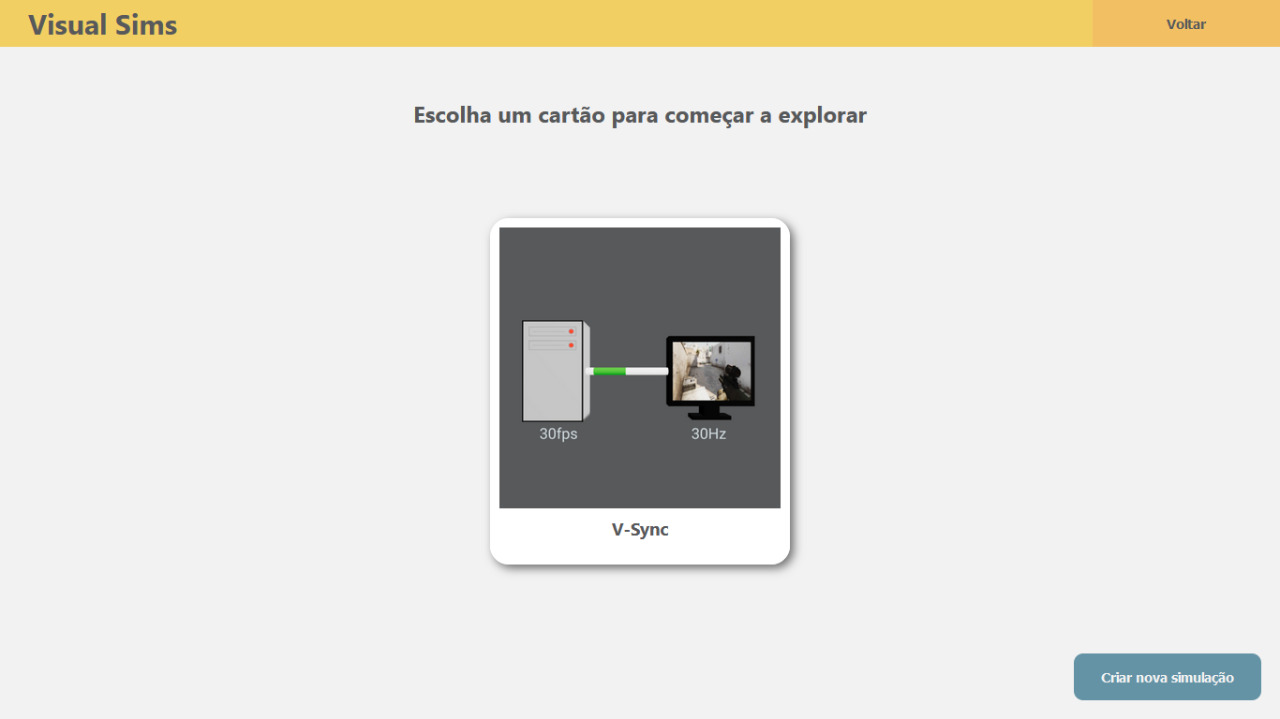
\includegraphics[scale=.2]{Navegacao/pagina_galeria.jpeg}
  \caption{Galeria de Simulações}
  \label{galeria}
\end{figure}

\begin{figure}[htbp]
  \centering 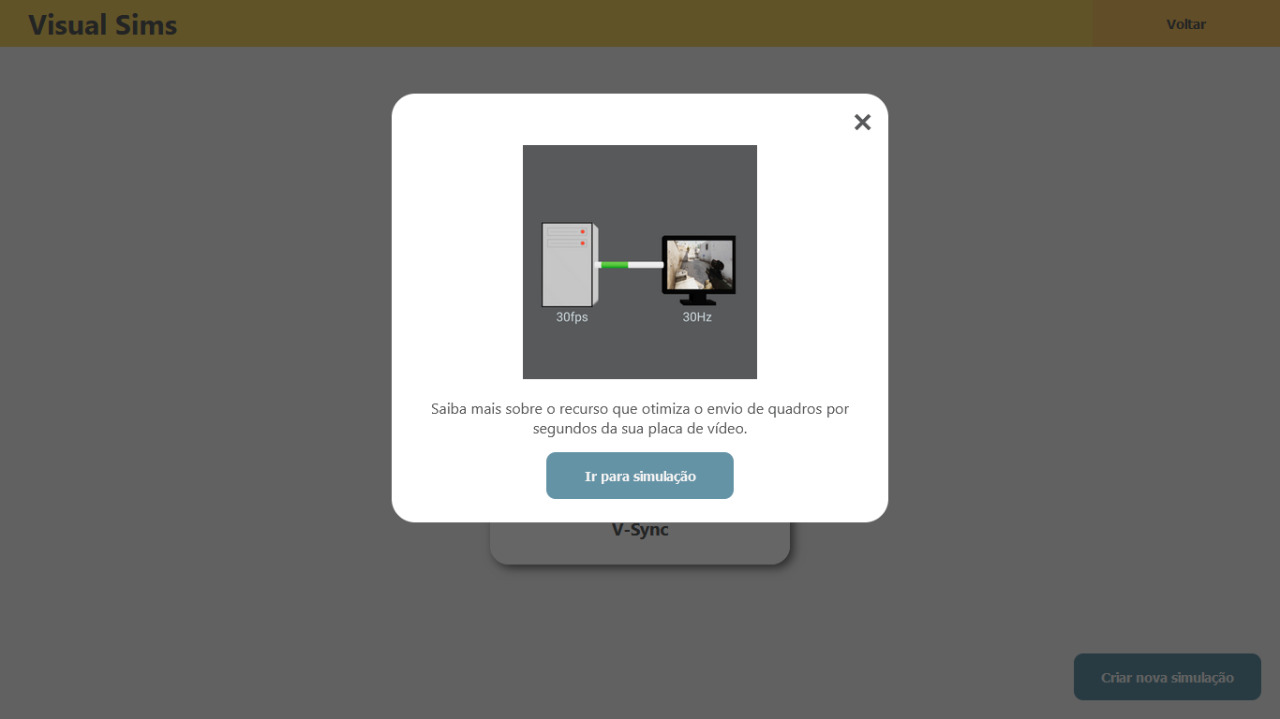
\includegraphics[scale=.2]{Navegacao/card_galeria.jpeg}
  \caption{Mais informações}
  \label{card_galeria}
\end{figure}

Após a escolha da simulação desejada o usuário é redirecionado para a página contendo o modelo da simulação, figura~\ref{simulacao}. Na página de simulação o usuário pode interagir com o ambiente, explorando o painel à direita que contém uma explicação sobre a simulação e os controles que fazem alterações na simulação para complementar a explicação. 

\begin{figure}[htbp]
  \centering 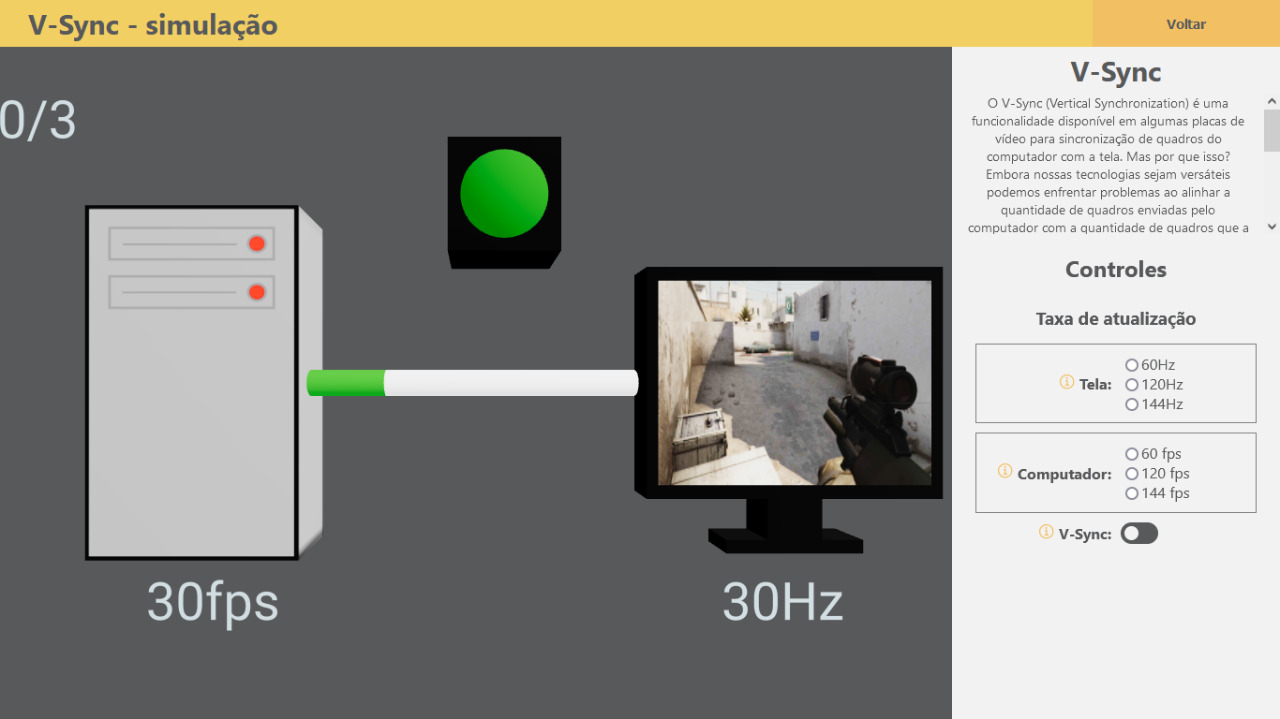
\includegraphics[scale=.2]{Navegacao/pagina_simulacao.jpeg}
  \caption{Simulação}
  \label{simulacao}
\end{figure}

As simulações não precisam ser controladas somente pelo painel, também é possível adicionar funcionalidades dentro da janela dos modelos 3D, como ao passar o mouse e aparecer mais informação sobre a simulação, figura~\ref{simulacao_extra}. 

\begin{figure}[htbp]
  \centering 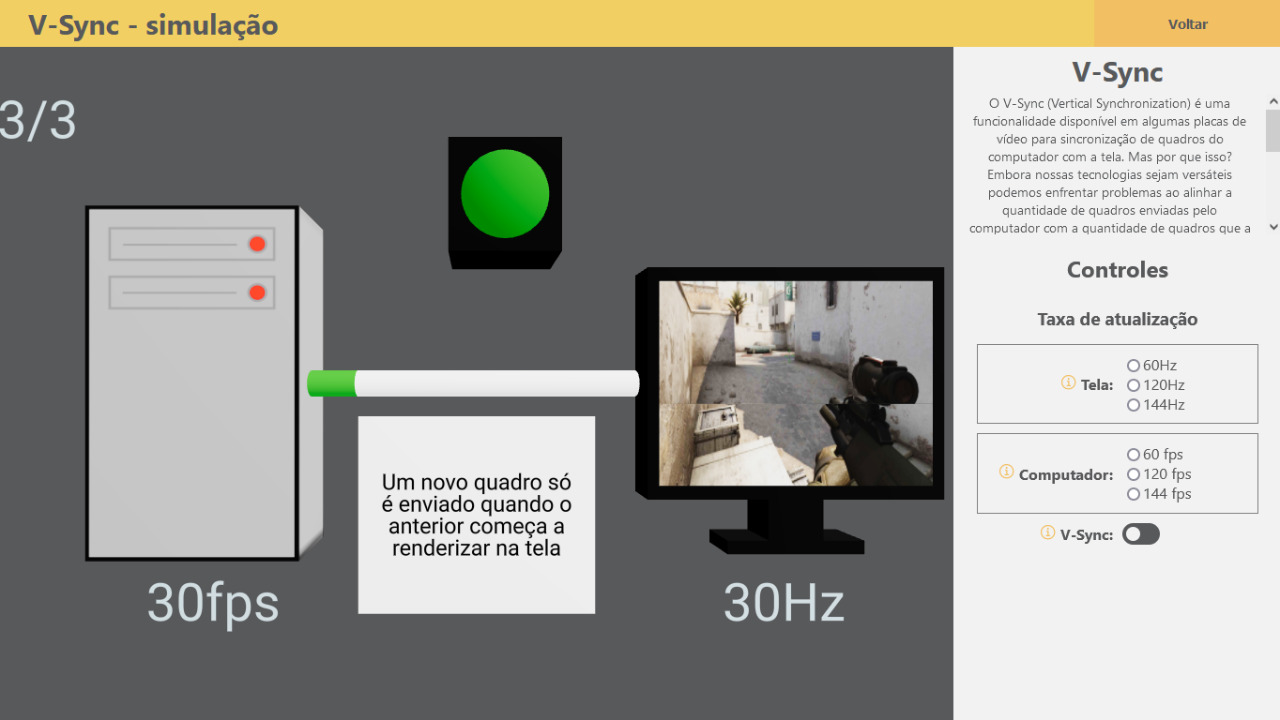
\includegraphics[scale=.2]{Navegacao/pagina_simulacao_extra.jpeg}
  \caption{Mais sobre a simulação}
  \label{simulacao_extra}
\end{figure}

\chapter{Desenvolvimento}
\label{cap: desenvolvimento}

Este capítulo é dedicado ao desenvolvimento da plataforma Visual Sims e uma breve discussão acerca das decisões que foram tomadas para o seu desenvolvimento. Abordando desde o levantamento dos dados necessários quanto as tecnologias utilizadas, apresentando suas vantagens frente ao projeto proposto.

A etapa de desenvolvimento teve como resultado um site desenvolvido para web, direcionado ao uso em desktop. A busca por informação deve ser livre, portanto uma plataforma web tem o potencial de atingir a maior parte do publico alvo. Outra vantagem de uma aplicação web é sua capacidade de criação, a tela do computador podendo ser comparada com uma tela em branco, em que tudo pode ser criado.

\section{Tecnologias}

O desenvolvimento de páginas estáticas tradicionais, com HTML e CSS, possibilitam a criação de diversos sites com diferentes propósitos, com a utilização da API WebGL as possibilidades de criação aumentam ainda mais. A combinação de JavaScript com WebGL criam uma ferramenta adaptável ao usuário da web.

Além de pensar na parte gráfica, é necessário levar em consideração a parte estrutural do projeto como um todo. Uma tecnologia que se mostrou bastante compatível com WebGL, e demonstrou ser bem estruturada, é a biblioteca React. Outra vantagem de escolher React é que por ser uma tecnologia bem atual é fácil de encontrar documentação e suporte na comunidade.

\subsection{WebGL}

WebGL é uma API em JavaScript que utiliza o elemento Canvas do HTML5 para renderização de elementos 2D e 3D. Esta API é uma evolução da API OpenGL, responsável por unificar 

Uma API é um conjunto de funções que tem como principal objetivo fazer a comunicação do software com o hardware. Dessa forma a API de WebGL além de fornecer funções que tornam a programação 2D e 3D mais prática, faz isso de uma forma mais otimizada, permitindo o acesso do navegador ao uso da GPU do computador. 

Para entendermos melhor em que momento o WebGL atua, precisamos entender o fluxo de criação de um objeto em uma cena. Este processo é composto de diversas etapas, e muitas delas não necessitam de alterações. Na figura~\ref{pipeline_grafico} podemos ver o pipeline de redenrização.

\begin{figure}[htbp]
  \centering 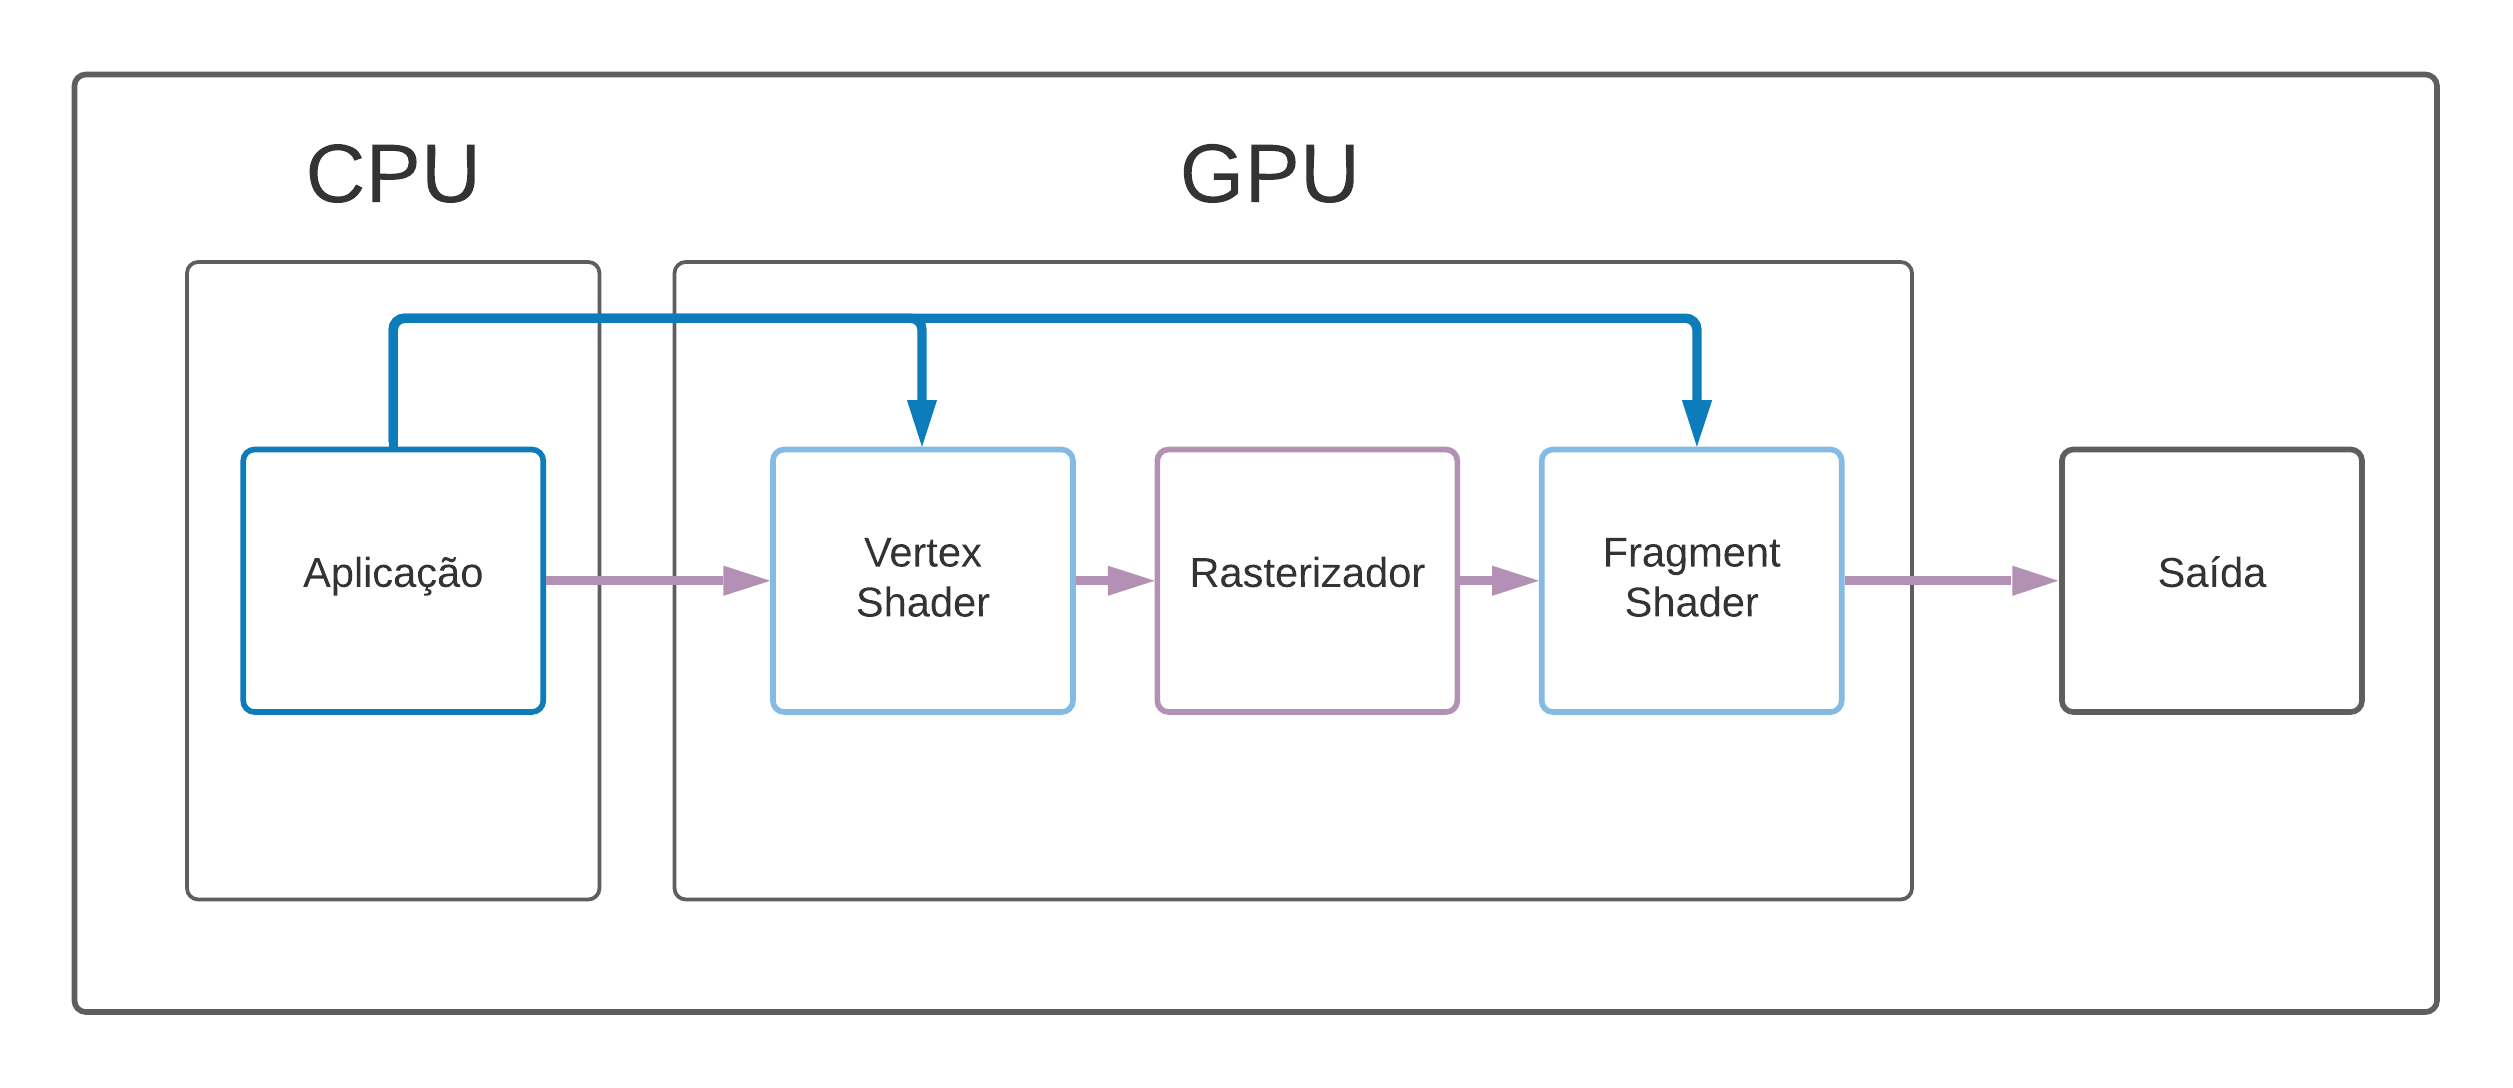
\includegraphics[scale=.7]{pipeline_grafico}
  \caption{Pipeline Gráfico}
  \label{pipeline_grafico}
\end{figure}% todo melhorar a imagem, colocar as outras etapas

Começando o processo de renderização a primeira etapa passar pelo Vertex Shader, ele é responsável por receber um conjunto de vértices definidos na aplicação e enviar para o rasterizador estes vértices mapeados. O Rasterizador por sua vez tem o papel de transformar os vértices em pixels, para que assim o Fragment Shader possa colorir eles.

Na figura podemos observar destacado em azul as etapas que são programáveis. São elas que recebem o suporte do WebGL. As setas em roxo representam o fluxo de dados durante a execução do programa. 

Portanto, o WebGL fornece suporte para a criação do Vertex Shader, com a utilização da linguagem JavaScript, e o Fragment Shader, utilizando a linguagem GLSL. 

\subsection{React}

React é uma das bibliotecas para JavaScript mais utilizadas na criação de novos projetos web da atualidade. A sua popularidade se dá pela sua estrutura e reusabilidade. Dentro do React é possível criar estruturas modulares que serão reaproveitadas em diversas partes do projeto. 

Criando um componente como uma classe é possível chamar ela dentro de novos componentes e aproveitar tanto a parte funcional de JavaScript quanto o layout do componente construído com HTML. Entretanto essa não é a principal função do React. Se baseando no controle de estados, os Hooks, o React tem um alto controle do que está sendo renderizado na tela. Fazendo assim a integração com elementos gráficos algo mais trivial.

\subsection{Three.js}

Three.js é uma biblioteca que abstrai algumas declarações que precisariamos fazer utilizando somente JavaScript e GLSL para programação em WebGL. 

\subsection{React Three Fiber}

React Three Fiber é a biblioteca que facilita a programação utilizando Three.js e React. Ela permite a criação de componentes 3D reutilizáveis dentro da aplicação.

\section{Coleta de dados}

Para o desenvolvimento da plataforma Visual Sims foi necessária uma coleta de dados acerca das simulações que seriam apresentadas como exemplo. O modelo de simulação desenvolvido foi sobre o recurso V-Sync, conceito que não consta no currículo dos cursos de computação, mas possibilita um melhor entendimento sobre o conceito de frames por segundo. Além de ter uma visão de renderização além de apenas um quadro.

A seguir irei aprofundar os conhecimentos sobre o recurso e falar sobre a vantagem de apresentar como conteúdo extra.

\subsection{V-Sync}

O V-Sync (Vertical Synchronization) é uma funcionalidade disponível em algumas placas de vídeo para sincronização de quadros do computador com a tela. Embora nossas tecnologias sejam versáteis podemos enfrentar problemas ao alinhar a quantidade de quadros enviadas pelo computador com a quantidade de quadros que a tela recebe.

Essa diferença se torna um problema quando é possível ver uma quebra no quadro. Essa quebra ocorre porque a velocidade de renderização do quadro atual é diferente da velocidade em que os quadros estão chegando. Sendo a renderização ser feita de cima para baixo, enquanto um quadro está terminando de renderizar o próximo já inicia o processo, por isso acaba parecendo um corte na tela horizontalmente.

Para resolver este problema o V-Sync sincroniza o número de quadros enviados ao monitor de acordo com a sua capacidade, enviando um quadro somente quando o monitor estiver pronto para recebe-lo. Ao analisarmos o V-Sync também devemos levar em consideração que outros fatores podem atrasar o envio do quadro, como o processamento de cada quadro, e dessa forma parecer que o V-Sync na verdade faz baixar o fps. 


\section{Criação do Projeto}

Para o desenvolvimento do projeto então foi utilizada a combinação da biblioteca React juntamente com a React Three Fiber, para criar um projeto modular e reutilizável. Além de modular, essas tecnologias facilitam o desenvolvimento, pois tornam o código legível e de fácil entendimento, afim de diminuir a curva de aprendizado da estrutura do projeto.

Uma decisão de projeto importante é a forma de estruturação das pastas. Como em React o objetivo principal do projeto é criar componentes reutilizáveis, é ainda mais importante manter uma boa organização das pastas. Com isso em mente foi adotado para o projeto o Atomic Design. Que consiste em subdividir os componentes em Atomos, Moleculas e Organismos, dessa forma é fácil de encontrar os componentes desejados e de forma intuitiva criar novos componentes.

\chapter{Resultados e Discussões}
\label{cap: resultados_e_discussoes}

O resultado do desenvolvimento traz uma plataforma que atende ao esperado. Entretanto, a ideia inicial do projeto seria criar uma ferramenta dentro do site que permitisse a criação de novas simulações sem precisar realizar a programação do front-end. Infelizmente durante a fase de prototipação foram encontradas algumas dificuldades acerca de criar esta ferramenta dentro do prazo previsto. Um protótipo do que seria essa funcionalidade foi criado, figura~\ref{prototipo_criar_simulacao}. 

Sendo o foco do projeto criar uma plataforma que disponibilize exemplos visuais para auxiliar no ensino, o resultado está de acordo com o proposto. Por meio de utilização dos componentes e estruturas já criadas o desenvolvimento de uma nova simulação se dá de forma mais simples. O código está disponível e público para estudo e desenvolvimento.

\begin{figure}[htbp]
  \centering 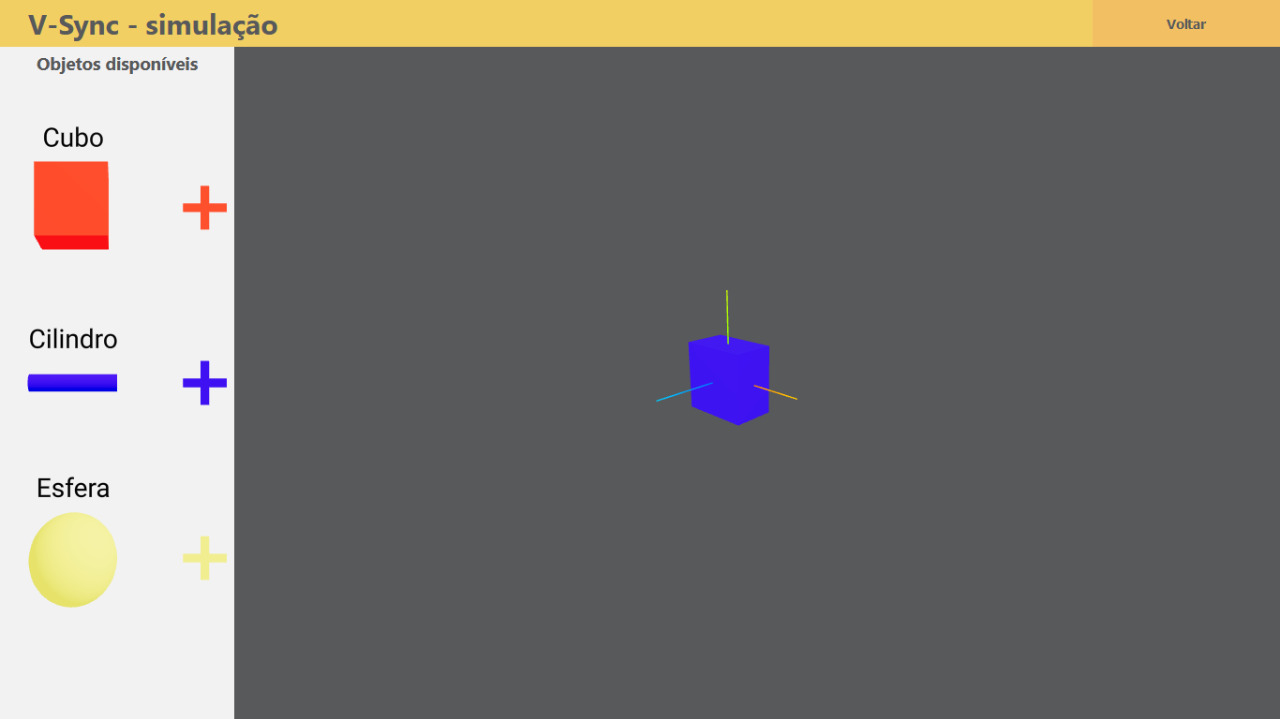
\includegraphics[scale=.2]{Navegacao/pagina_criar_simulacao.jpeg}
  \caption{Protótipo para criar simulação}
  \label{prototipo_criar_simulacao}
\end{figure}

Com base em pesquisas informais, foi constatado que o site oferece um resultado positivo, por meio de testes os usuários puderam aprimorar seus conhecimentos sobre o conteúdo apresentado. Foram levantados pontos de melhora em questão de de usabilidade, como para alguns não é possível ver a barra de rolagem do texto explicativo, figura~\ref{antes_texto_explicativo} e figura~\ref{melhoria_texto_explicativo} , por configuração de sistemas operacionais. Este tipo de avaliação demonstra que os usuários estavam envolvidos com a aplicação e também que a plataforma têm potencial para demonstrar o interesse deles.

\begin{figure}[htbp]
  \centering 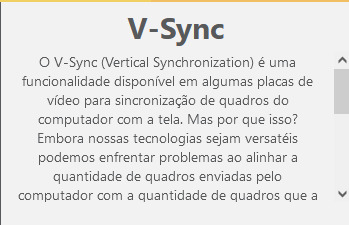
\includegraphics[scale=.3]{Navegacao/antes_texto_explicativo.jpeg}
  \caption{Texto explicativo antes da melhoria}
  \label{antes_texto_explicativo}
\end{figure}

\begin{figure}[htbp]
  \centering 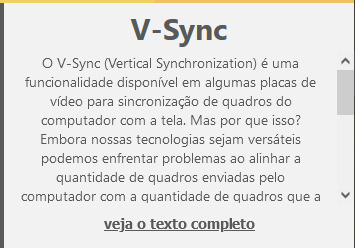
\includegraphics[scale=.3]{Navegacao/melhoria_texto_explicativo.jpeg}
  \caption{Texto explicativo após melhoria}
  \label{melhoria_texto_explicativo}
\end{figure}

\section{Formulário teste}

\chapter{Conclusão}
\label{cap: conclusao}

O trabalho desenvolvido têm como objetivo de ajudar 

\bibliographystyle{abnt}
\bibliography{bibliografia} 

% Apêndices (Opcional) - Material produzido pelo autor
% \apendices
% \chapter{Um Apêndice}

% Anexos (Opcional) - Material produzido por outro
% \anexos
% \chapter{Um Anexo}

% \chapter{Outro Anexo}

% Faz a capa do CDROM
% \makecover

\end{document}

